\usepackage{url}
\section{Dokumentengeschichte}
\begin{table}[h]
 \begin{tabular}{|l|l|p{4cm}|}
 \hline
 Zeitraum & PL/Autor(en) & Änderungen \\
 \hline
 Wintersemester 2017/2018 & Justin Sprenger (s0556255) & 
text \newline 
text \newline 
text \newline 
text \newline 
text \newline 
text \newline 
 
  \\
 \hline
 \end{tabular}
 \caption{Dokumentengeschichte}
 \end{table}

\section{Aufgabe der Komponente}
Verbale kurze prägnante Beschreibung, was die Komponente leisten soll.
Das sind wenige Seiten.

(Ausfüllen in Prototyp-Phase)

Der Android-Editor soll dem Nutzer die Möglichkeit bieten alte historische Orte aufzuzeichnen. Die App soll die von dem Nutzer abgelaufenen Strecken/Gebite aufzeichnen und abspeichern. Die aufgezeichneten Daten sollen als GeoJSON gespeichert werden und anschließend in die Datenbank eingefügt werden, damit diese anschließend für jeden und nicht nur auf dem lokalem Gerät sichtbar sind. Die gespeicherten Daten sollen des weiteren Mit Namen und Zeitstempel versehen werden.

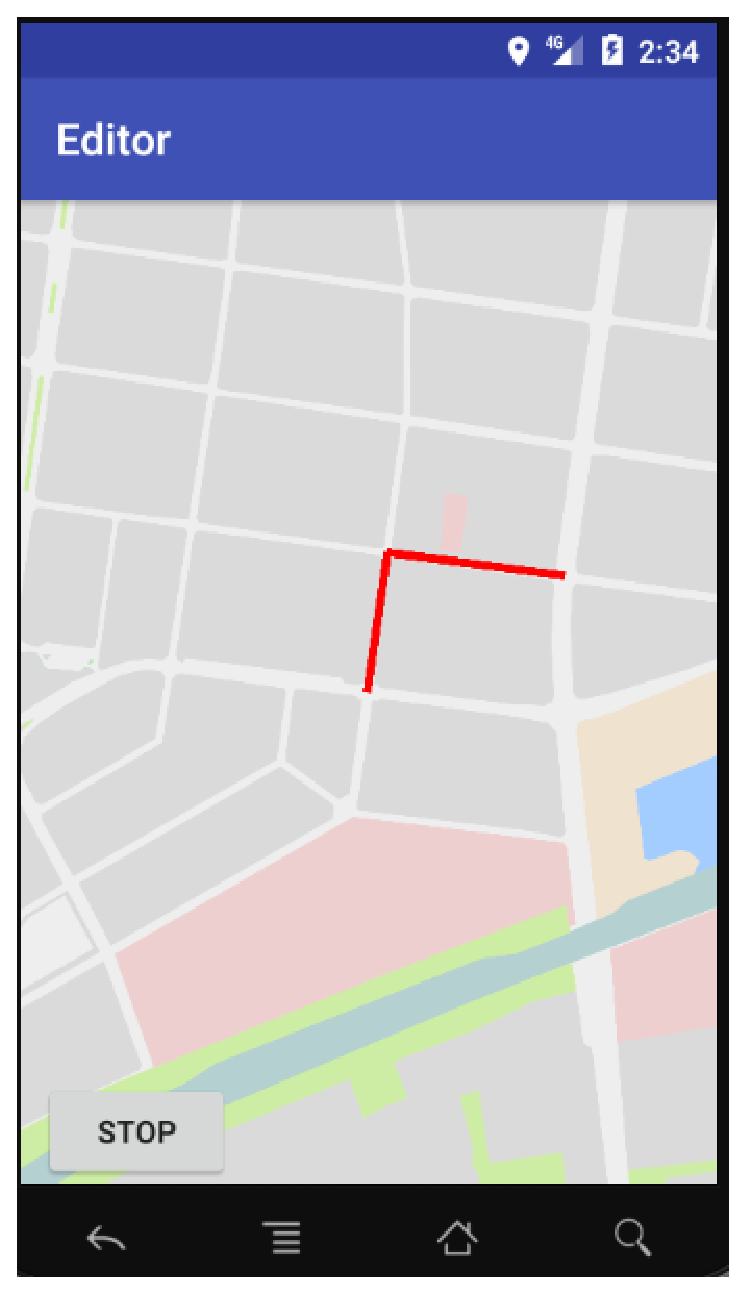
\includegraphics[width=0.45\textwidth]{AndroidEditorOV}

\section{Architektur}

\subsection{Überlick}
Grafik der Teile der Komponente (wichtig: Benennung aller Schnittstellen). 
Anwendung der Komponente nennen (Use Case).

Übliche Interaktionen durch Interaktionsdiagramme.

(Ausfüllen in Prototyp-Phase)

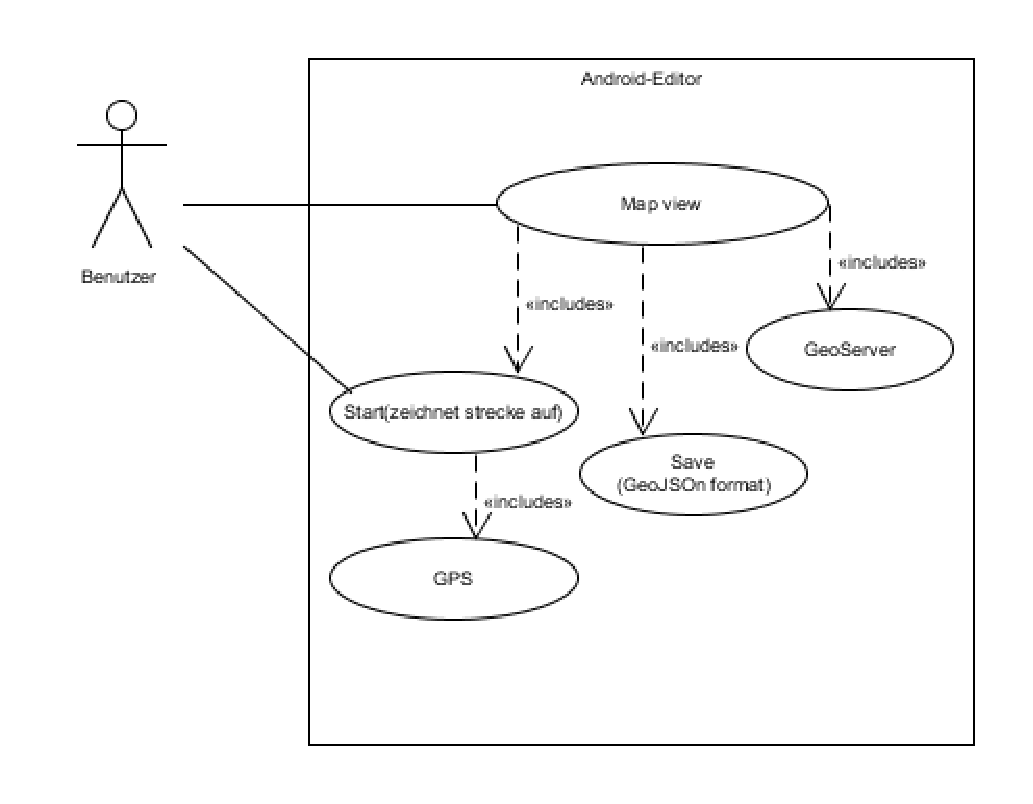
\includegraphics[width=0.45\textwidth]{UseCase}

Der Editor bietet keine Schnittstellen nach außen. Jedoch soll die Import Schnittstelle verwendet werden um die Aufgezeichneten Daten der OHDM Datenbank hinzuzufügen.

Der Editor lädt sich die Layer, welche für die OHDM Map benötigt werden, von dem Geo-Server und erzeugt mithilfe der OSMdroid-Api eine Karte auf dem Smartphone. Der Nutzer hat die Möglichkeit eine Strecke oder ein Gebiet aufzuzeichnen und abzuspeichern. Des weiteren soll ein Zeitstempel und ein Name angegeben werden können um Historische Orte zu dokumentieren.

Die aufgezeichnete Strecke wird auf der Karte als Rote Linie Dargestellt, welche sich kontinuierlich wärend der aufzeichnungs-Phase verändert. Der Nutzer hat anschließend die Möglichkeit anzugeben um was es sich handelt (Gebiet,Punkt,Strecke). Die aufgezeichneten Datene werden als GeoJSOn zwischengespeichert und sollen anschließend an die Import-Schnitstelle übertragen werden.

\subsection{Schnittstellendefinitionen}

Diese Anwendung bietet keine Schnittstellen nach außen.

\subsection{genutztes Komponenten}
Beschreibung, welche weiteren Komponenten (in welchen Versionen, wo beziehbar) genutzt werden.

(Beginnen in Prototyp-Phase. Konkretisieren in der Alphaphase)

Momentan wird die OSMdroid-Api verwendet um die OHDM-Karte darzustellen.
Die App soll in einer Späteren Version die Import-Schnittstelle verwenden um die aufgezeichneten Daten(Koordinaten) zu übertragen.

\section{Nutzung}
\subsection{Code}
Der Code befindet sich auf GitHub. \url{https://github.com/OpenHistoricalDataMap/OHDMAndroidEditor/}
Die verwendete IDE ist Android Studio.

\subsection{Deployment / Runtime}
Mittels der IDE Android Studio kann die App in einem Emulator gestartet oder direkt auf ein Device installiert werden.

\section{Qualitätssicherung}

App ist noch Sehr fehleranfällig, stürzte häufig ab, seit dem der stacked Layer eingefügt wurde stürzt die app kaum noch ab. Der Editor ist Momentan noch ein Prototyp.
Großteil der Fehler die Auftreten können werden abgefangen.

\subsection{Test}
Wie wird die Komponente getestet.

Getestet wir die Software durch manuell simulierte GPS Daten, und durch real abgelaufene strecken.

\section{Vorschläge / Ausblick}
Was ist aufgefallen, was sollte man ändern? Löschen Sie auch gern die Kommentare
der Vorgänger, aber nur, wenn es wirklich nicht mehr relevant ist.

Anfänglich gab es Probleme mit dem Laden der Layern. Die Ladezeit hatte für ein Gebit fast 5 Minuten gedauert und es kam zu vielen Exceptions. Die Exceptions traten auf da für einige Koordinaten keine Layerdaten/Bilddaten existierten(vermutlich zu genaue Koordinaten). Durch den StackedLayer(Multilayer) wurde dieses Problem gelöst. Die Ladezeit ist nun annehmbar(ca 1 Minute) und es treten kaum bis keine Exceptions auf.

Die aufgezeichneten Strecken sind sehr genau und es treten viele kleine Abweichungen auf. Aus diesem Grund wurde wurde eine Abweichungsbegrenzung von 1 Meter gesetzt. Alle Koordinaten welche eine Abweichung von weniger als 1 Meter von den vorher aufgezeichneten Koordinaten haben werden ignoriert und nicht aufgezeichnet.

Bisher ist noch nicht die Import-Schnittstelle eingebunden, das heißt die Daten werden bisher nicht in die Datenbank übernommen, jedoch schon ins GeoJSON-Format umgewandelt und testweise auf dem Display mit ausgegeben.

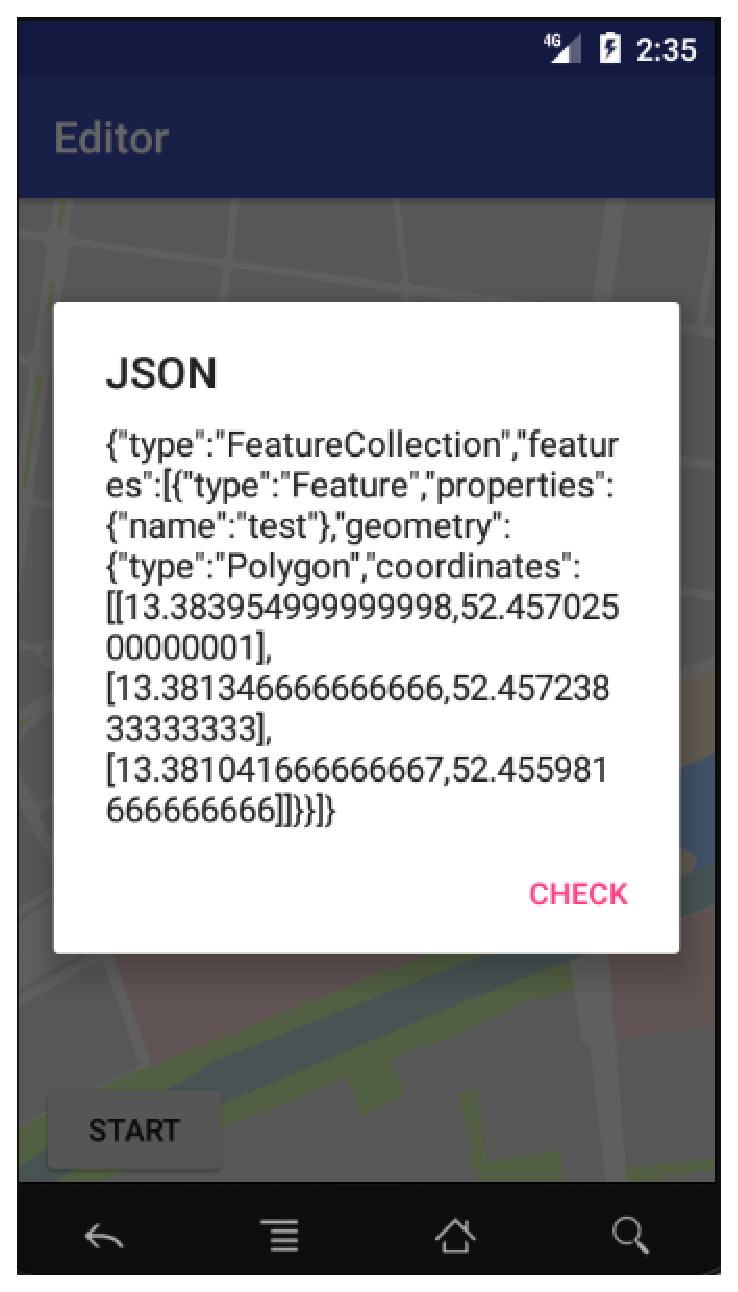
\includegraphics[width=0.45\textwidth]{AndroidEditorJSON}
